%% Requires compilation with XeLaTeX or LuaLaTeX
\documentclass[10pt,xcolor={table,dvipsnames},t]{beamer}
\usetheme{UCBerkeley}
\usepackage[export]{adjustbox}

\title[Your Short Title]{Проектная работа}
\subtitle{Высокоэффективное сетевое программирование на языке Swift}
\author{Андрей Козырев \\ \small Руководитель: Виталий Брагилевский}
\institute{Санкт-Петербургский Государственный Университет. Факультет математики и компьютерных наук. Современное программирование}
\date{24 мая 2022}

\begin{document}

\begin{frame}
  \titlepage
\end{frame}

% Uncomment these lines for an automatically generated outline.
%\begin{frame}{Outline}
%  \tableofcontents
%\end{frame}

\section{Введение}

% \begin{frame}{Введение}

% Исследование посвящено изучению вопроса компетентности языка \texttt{Swift} для написания высокоэффективных серверов с большим потоком длительных подключений.

% В рамках исследования был выбран фреймворк \texttt{SwiftNIO} и аналогичный ему фреймворк \texttt{Netty} на языке \texttt{Java}. 

% \end{frame}

\begin{frame}{Задачи}

\begin{itemize}
  \item Определить аналоги в других языках.
  \item Изучить качество поддержки, скорость развития, интерфейс и возможности \texttt{SwiftNIO}. 
  \item Разработать сюжеты тестирования клиент-серверных приложений.
  \item Проанализировать производительность относительно \texttt{Netty}.
  \item Выявить сильные и слабые стороны фреймворка. 
  \item Сделать выводы о конкуренто-способности Swift, и, в частности \texttt{SwiftNIO} для написания серверных приложений. 
\end{itemize}

\end{frame}

\subsection{Общие черты}

\begin{frame}{SwiftNIO в общих чертах}

\texttt{SwiftNIO} это асинхронный, кросс-платформенный событийно ориентированный фреймворк для написания высокоэффективных серверов и~клиентов. 

\begin{block}{``It's like Netty, but written for Swift''.}
Над фреймворком во многом работала команда, разрабатывавшая \texttt{Netty}. Он~новый, стремительно развивается, и активно поддерживается. 

\end{block}

\end{frame}

\smallframetitle

\begin{frame}{Преимущества}

\begin{itemize}
\item Схожесть интерфейса с \texttt{Netty}. Удобство использования. 
\item Возможность написания как серверной, так и клиентской части. 
\item Неблокирующий \texttt{IO}. 
\end{itemize}

\end{frame}

\begin{frame}{Недостатки}

\begin{itemize}
\item Незаконченная работа над реализацией \texttt{UDP}.
\item Интерфейс во многом заимствует конструкции, являющиеся на данный момент \texttt{deprecated} в \texttt{Java}. 
\end{itemize}

\end{frame}

\begin{frame}
\frametitle{Разработанная инфраструктура}

\begin{itemize}
\item Написаны максимально близкие по реализации сервера на \texttt{SwiftNIO} и \texttt{Netty}.
\item Написан клиент на \texttt{SwiftNIO}.
\item Разработан набор скриптов на \texttt{Python}, собирающий и запускающий все компоненты и позволяющий протестировать работу серверов, получив данные в~графическом виде.
\end{itemize}
\end{frame}

\section{Метрики}

\begin{frame}
\frametitle{Количество информации, получаемое клиентом}

\begin{center}
    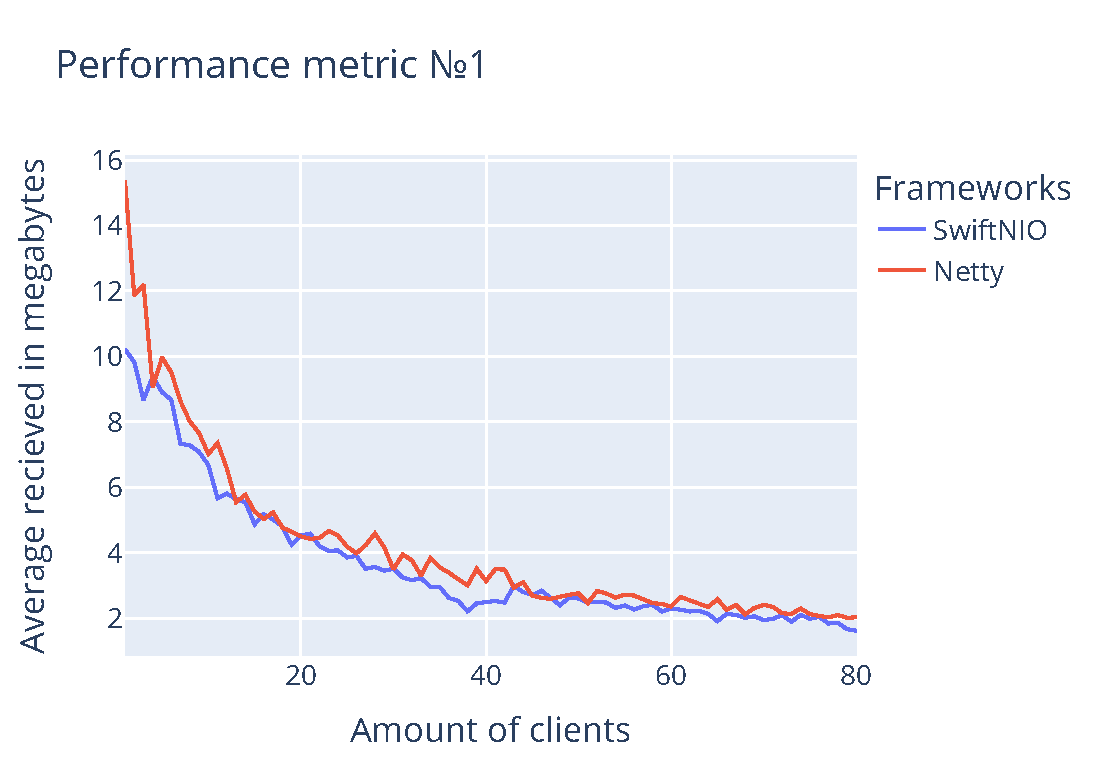
\includegraphics[width=.65\textwidth,height=.65\textheight]{metric1_final.pdf}
\end{center}
\end{frame}

\begin{frame}
\frametitle{Отклонение от среднего}

\begin{center}
    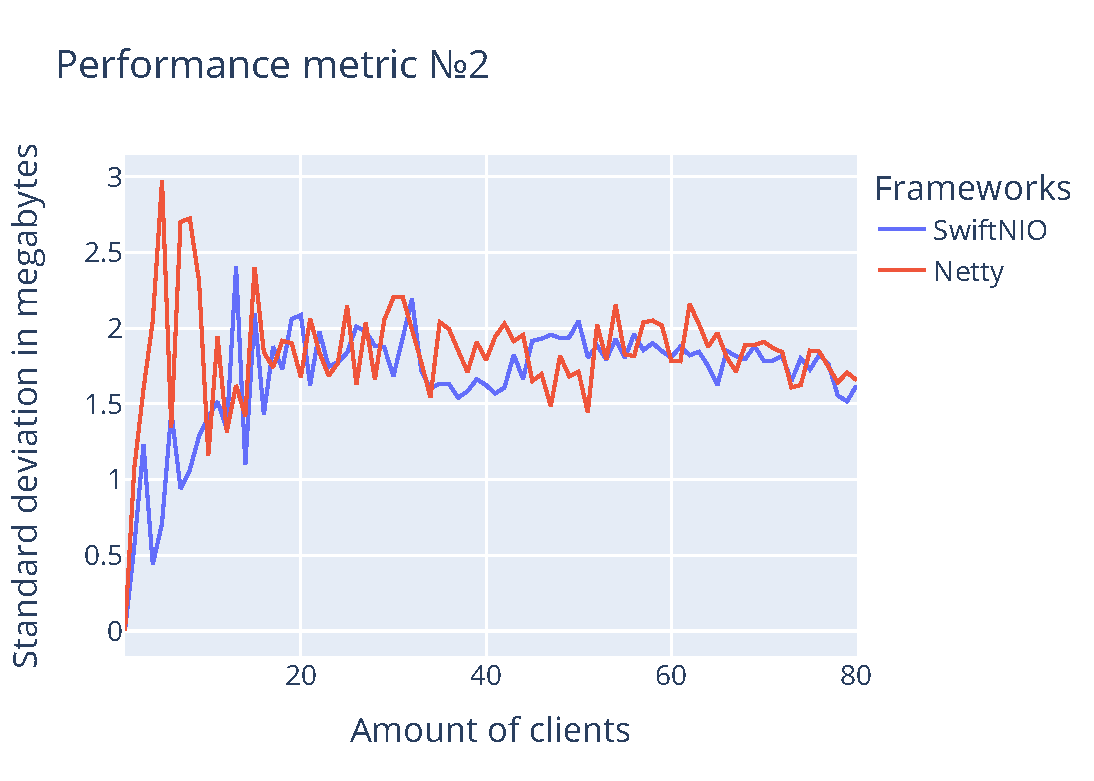
\includegraphics[width=.65\textwidth,height=.65\textheight]{metric2_final.pdf}
\end{center}
\end{frame}

\begin{frame}
\frametitle{Нагрузка на процессор}

\begin{center}
    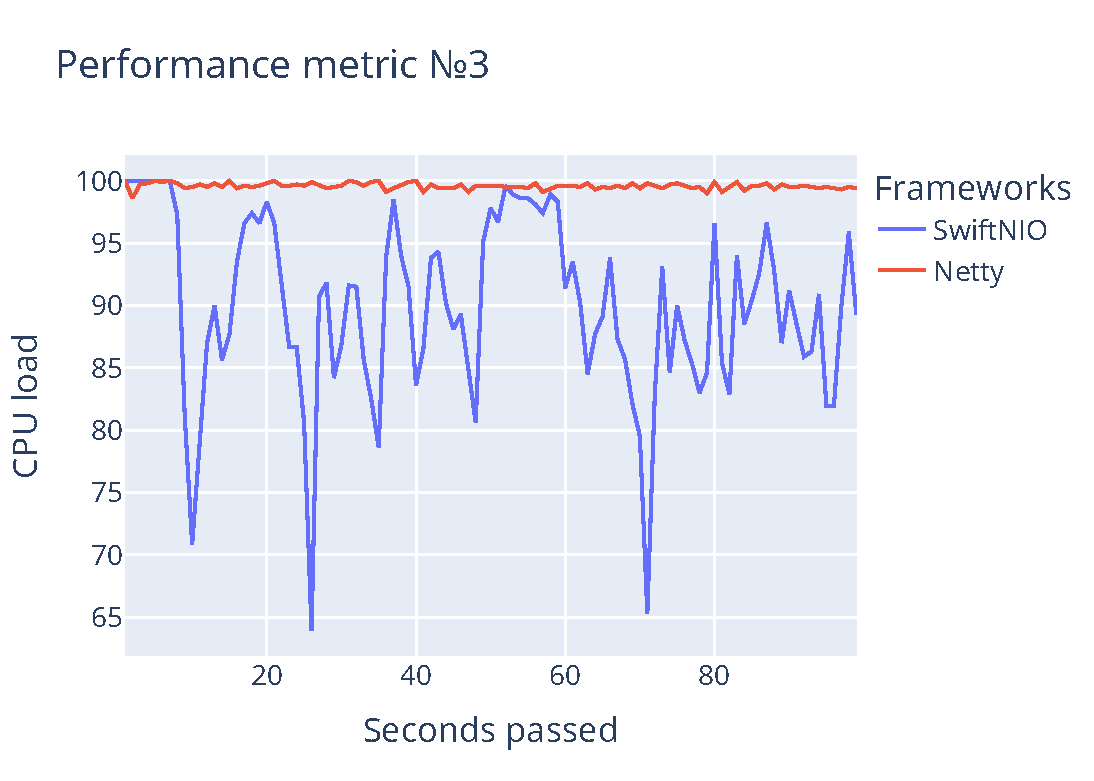
\includegraphics[width=.65\textwidth,height=.65\textheight]{metric3_final.pdf}
\end{center}
\end{frame}

\normalframetitle

\begin{frame}
\frametitle{Резюме}
\begin{itemize}
  \item Разработаны сюжеты и инструменты тестирования серверных приложений.
  \item Выявлена конкуренто-способность \texttt{Swift} для сетевого программирования.
  \item Выявлены слабые места \texttt{SwiftNIO}. 
  \item Можно предположить, что \texttt{SwiftNIO} использует более современные системные вызовы, которые отдают много работы операционной системе. 
\end{itemize}
\vspace{0.6cm}

\includegraphics[scale=0.14,right]{swift_logo_qrcode.png}


\end{frame}


\end{document}
